Recent approaches to knowledge-intensive NLP tasks combine neural network based models with a retrieval component that leverages dense vector representations \citep{guu2020realm,lewis2020retrieval,petroni2021kilt}.
The most straightforward example is question answering, where the retriever receives a question as an input and returns relevant documents to be used by the reader (both encoder and decoder), which outputs the answer \citep{nadeem2019fakta,chen2020neural}.
The same approach can also be applied for models for other tasks, such as fact-checking \citep{tchechmedjiev2019claimskg}, retrieval-enhanced language modelling \citep{logan2019baracks,borgeaud2021improving,he2021efficient}, or knowledgable dialogue \citep{dinan2018wizard,wu2020topicka}.
Moreover, this paradigm can also be applied to systems that utilize e.g. caching of contexts from the training corpus to provide better output, such as the k-nearest neighbours language model proposed by \citet{khandelwal2019generalization} or the dynamic gating language model mechanism by \citet{yogatama2021adaptive}.
All these pipelines are generalized as retrieving an artefact from a knowledge base \citep{zouhar2021artefact} on which the reader is conditioned together with the query.
Overall, they represent a trend of combining the advantages of non-parametric (scalability, auditability) and non-parametric models (performance, automatic optimization).

Crucially, all of the previous examples rely on the quality of the retrieval component and the knowledge base.
The knowledge base is usually indexed by dense vector representations\footnote{Sparse representations via BM25 \citep{robertson1995okapi} are also commonly used but not the focus of this work.} and the retrieval component performs maximum similarity search, commonly using the inner product or the $L^2$ distance, to retrieve documents\footnote{We refer to the retrieved objects as documents though they commonly range from spans of text (e.g. 100 tokens) to the full documents.
    This is explained and disambiguated in \Cref{chapter:splitting_filtering}.} from the knowledge base.
Only the index alone takes up a large amount of size of the knowledge base (150GB), making deployment and experimentation very difficult.\footnote{For experimenting with this index, a memory of up to 1TB is required.}
The retrieval speed is also dependent on the dimensionality of the index vector.
An example of a large knowledge base is the work of \citet{borgeaud2021improving} which performs retrieval over a database of 1.8 billion documents.

The possible impacts of reducing the knowledge base size are (1) reduced deployment and research constraints and (2) improved retrieval efficiency.
The constraints are retaining as much of the original retrieval performance as possible.
This thesis focuses on the issue of compressing the knowledge base size primarily through the dimensionality and precision reduction of the index and makes the following contributions:

\begin{itemize}
    \item Analysis of negative results of various splitting and filtering methods.
    \item Comparison of various unsupervised index compression methods in retrieval experiments, including random projections, PCA, autoencoder, precision reduction and their combination. % They can be universally applied to knowledge-intensive NLP tasks. 
    \item Examination of effective pre- and post-processing transformations, showing that centering and normalization are necessary for boosting the performance.
    \item Analysis on the impact of adding irrelevant documents and retrieval errors. Recommendations for use by practitioners.
\end{itemize}

This thesis is split into two main chapters: introduction to the problem and negative results of Splitting \& Filtering (\Cref{chapter:splitting_filtering}) and Dimension Reduction (\Cref{chapter:dim_reduction}, the primary content of this thesis).
We provide further analysis in \Cref{sec:analysis} and conclude with usage recommendations in \Cref{chapter:discussion}.

The repository for this thesis is available open-source.\footnote{
    \href{https://github.com/zouharvi/kb-shrink}{github.com/zouharvi/kb-shrink}
}

\section{Related Work}

This thesis is largely based on two papers written by the same author: \citet{zouhar2021artefact,zouhar2022knowledge} with a more detailed background and \Cref{chapter:splitting_filtering} added.

\paragraph{Knowledge-intensive NLP Overview.}

A comprehensive overview of earlier work on neural model-based information retrieval systems together with a general introduction has been done by \citet{mitra2017neural}.
More recently models such as BERT have been utilized successfully for the task of retrieval itself \citep{nogueira2019multi, soleimani2020bert}.

The aim of KILT \cite{petroni2021kilt} is to provide a common knowledge base for a number of different NLP tasks (ranging from question answering to fact verification) and to stimulate research in task-agnostic memory architectures. Reformulating various NLP tasks to all use the same knowledge base format provides a stepping stone for the formalisms of artefact retrieval.

Defining a task-agnostic abstract model is closely related to multi-task learning.
The goal of this approach is to improve the performance by training the model on multiple tasks rather than on individual ones \citep{maillard-etal-2021-multi}.
The hope is that representations and generalizations learned for one task will help on another one and vice versa. A strong requirement for this is that the instantiations for different tasks (in the multi-task setup) share significant portions of the model.

An edge-case of this is using a pre-trained BERT model and then fine-tuning it for the new task and/or possibly adding extra layers to match the input and output shapes. Even for BERT, however, it was shown several times \cite{petroni2021kilt,liu2019multi,sun2019fine,kim2019qe} that training on multiple tasks improves the performance \citep{aghajanyan2021muppet}.
This would not be possible without a common model shared among the tasks.
Further related work is discussed in the respective sections when presenting individual NLP models and how they fit into this schema.

\paragraph{Reducing index size.}

A thorough overview of the issue of dimensionality reduction in information retrieval in the context of dual encoders has been done by \citet{luan2020sparse}.
Though in-depth and grounded in formal arguments, their study is focused on the limits and properties of dimension reduction in general (even with sparse representations) and the effect of document length on performance.
In contrast to their work, this thesis aims to compare more methods and give practical advice with experimental evidence.

A baseline for dimensionality reduction has been recently proposed by \citet{izacard2020memory} in which they perform the reduction while training the document (and query) encoder by adding a low dimensional linear projection layer as the final output layer. Compared to our work, their approach is supervised.

In the concurrent work of \citet{ma2021simple}, PCA is also used to reduce the size of the document index.
Compared to our work, they perform PCA using the combination of all question and document vectors. We show in \Cref{fig:pca_auto_main,fig:model_data} that this is not needed and the PCA transformation matrix can be estimated much more efficiently. Moreover, we use different unsupervised compression approaches for comparison and perform additional analysis of our findings.

An orthogonal approach to the issue of memory cost has been proposed by \citet{yamada2021efficient}.
Instead of moving to another continuous vector representation, their proposed method maps original vectors to vectors of binary values which are trained using the signal from the downstream task.
The pipeline, however, still relies on re-ranking using the uncompressed vectors.
This method is different from ours and in \Cref{subsec:prec_reduction} we show that they can be combined.

Finally, \citet{he2021efficient} investigate filtering and k-means pruning for the task of kNN language modelling. This work also circumvents the issue of having to always perform an expensive retrieval of a large data store by determining whether the retrieval is actually needed for a given input.

\paragraph{Effect of normalization.}

Normalization in information retrieval is historically connected with normalization with respect to the document length or term frequency \citep{khalid2008impact,na2015two,roy2018using}.
In the context of this thesis, we refer to vector normalization and in general post-processing functions for vectors.

\citet{timkey2021all} examine how dominating embedding dimensions can worsen retrieval performance.
They study the contribution of individual dimensions find that normalization is key for document retrieval based on dense vector representation when BERT-based embeddings are used.
Compared to our work, they study pre-trained BERT directly, while we focus on DPR.

\section{Retrieval pipelines}

Historically there has been a large focus on non-parametric models for knowledge-intensive NLP tasks.
Those are not models which don't have any parameters but rather they don't have a fixed amount of parameters.
This approach is particularly suited for tasks such as question answering because the knowledge is retrieved from a database and can be easily expanded or audited.
Opposed to that are models which store the knowledge in parameters, such as pre-trained language models, which became largely adopted in the NLP community.

The parametric models suffer from becoming outdated very quickly \citep{lazaridou2021pitfalls}, providing very little explainability in comparison to non-parametric models and performing poorly on unseen phenomena \citep{logan2019baracks}.
Recently there has been an emergence of the combination of these approaches, as shown in \Cref{tab:artefacts_summary}.
They work by retrieving something (\emph{artefacts}) from a knowledge base (or any persistent storage) and merging it in the computation of a parametric model.

An abstract pipeline in \Cref{fig:artefacts_diagram}, described in detail by \citet{zouhar2021artefact}, shows how these models operate.
The key components are \textit{encoder}, \textit{retriever}, \textit{aggregator} and \textit{model} (some may be joined together in some works, commonly the retriever and the aggregator).


\begin{figure*}[ht]
    \vspace{0.5cm}
    \center
    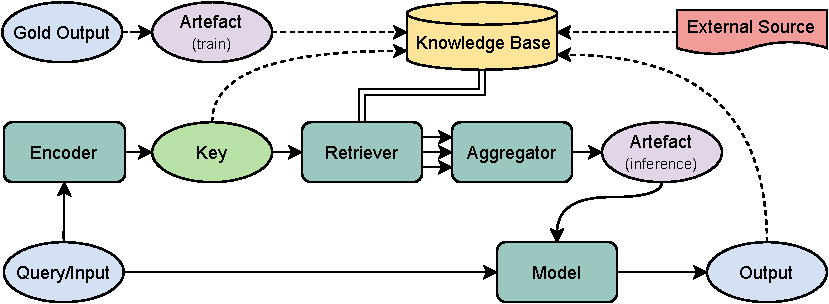
\includegraphics[width=\textwidth]{img/artefacts_diagram.pdf}
    \caption{General scheme of NLP models utilizing artefacts by retrieving them from a knowledge base and fusing them into the model in order to produce a better output. Dashed links are utilized only in knowledge base creation and usually not all at once.}
    \label{fig:artefacts_diagram}
\end{figure*}

The \textit{input} is specific to the given task.
For language modelling, it is the previous context, for question answering the question, for slot-filling usually the entity and the relation, and for fact-checking the fact to be verified.
In the context of this work, a \textit{knowledge base} is a collection of items, usually (but not necessarily) with a pre-built index that maps keys to values.
Prototypically, it is a collection of \textit{documents}, though it can also be a collection of gold training data input-output pairs or a knowledge graph.
\textit{Candidates} are values retrieved from the knowledge base, which may be later post-processed (e.g. reranking or averaging) by the aggregator to form an artefact.
\textit{key} is an object through which the retriever finds suitable artefacts. Commonly the key is a dense vector representation of the input, though it is not necessarily a vector and may be dependent also on an intermediate model computation.
An \textit{artefact} is an object which is (1) dependent on elements retrieved from the knowledge base (e.g. the concatenation of $k$ retrieved documents) and (2) can be used to improve the performance during training and inference. In the simplest example, it is the retrieved value itself, though it can also be multiple retrieved values or their combination.


In the context of question answering, we start with the query, then usually compute an embedding of it or use TF-IDF, then we give this to the retriever, which does maximum similarity search over a knowledge base, then the aggregator reranks and concatenates them and we get the artefact.
This is then fused into the model, for example, in the form of priming.
The model then produces the answer because it's conditioned both on the query and the artefact.

This formalism works also for other tasks that rely on retrieval, such as fact checking, knowledge base-enhanced language modelling or knowledgeable dialogue \citep{zouhar2021artefact}.
Most systems used in the literature differ in the encoder, retriever, and model design. We bring attention to four properties that characterize the differences between such systems.

% [itemsep=-0.24em]
\begin{itemize}
    \item \textbf{Fusion} (early, late, other)
    \item \textbf{Specificity} (sample, task, class)
    \item \textbf{KB source} (train, external, dynamic)
    \item \textbf{Key \& value type} (dense, sparse, other)
\end{itemize}

We consider the fusion mechanism to be of the highest interest.
Priming is very common with pretrained language modelling and is an example of an early fusion.
Formally the model estimates $p(y|x,\xi)$ where $y$ is the ground-truth output, $x$ is the query/input and $\xi$ is a retrieved artefact. Fusion \citet{sun2018open} concerns with which point is the artefact made available to the model. It can be presented to the model at the same time as the query/input, e.g. by concatenating $x$ and $\xi$ (early fusion), just before the output is created by the model (late fusion), or somewhere in between.
We can think of any model as a composition of functions $f_1, \ldots, f_n$.
% , one of which is also conditioned on the artefact.
% The model computation is a composition of functions $f_1, \ldots, f_n$.
In the simplest example of feed-forward networks, these correspond to single layers and activation functions and on a higher level, they correspond to whole encoder/decoder blocks. The distinction as to what counts as early and late is not clear and for presentation purposes, we consider early fusion at the level of $f_1$ and late fusion at the last stage, $f_n$. These functions themselves may, however, still be composed of multiple others. In \textbf{early fusion}, the artefact is the input together with the query to the first function $f_1$, while in \textbf{late fusion} the query is the single input to $f_1$ and artefact is considered only for $f_n$.
\begin{align*}
     & \text{No fusion:}           & f_n \circ \ldots \circ f_2 \circ f_1 (q)                              \\
     & \text{Early fusion:}        & f_n \circ \ldots \circ f_2 \circ f_1 (q, \xi)                         \\
     & \text{Late fusion:}         & f_n ( f_{n-1} \circ \ldots \circ f_1 (q), \xi)                        \\
     & \text{Intermediate fusion:} & f_n \circ \ldots \circ f_k ( f_{k-1} \circ \ldots \circ f_1 (q), \xi)
\end{align*}

Improvements for models for one task can also transfer to others.
This formalism also allows us to ask questions such as how do different fusion mechanisms affect the model computation.
The key component in all of these pipelines is retrieval.
This thesis focuses on a specific setup, described in \Cref{sec:intro_setup}, with the goal of reducing the knowledge base size.

See \Cref{appendix:fusion_discussion} for a discussion on .
For a description of specific systems and how they fit into this typology see the appendix in \citet{zouhar2021artefact}.

\begin{table*}[ht]
    \center
    \resizebox{\linewidth}{!}{%
    \setlength{\tabcolsep}{0.35em} % horizontal padding
    \renewcommand{\arraystretch}{1.5} % vertical padding
    \begin{tabular}{p{3.2cm}p{2.3cm}p{2.1cm}p{2.7cm}p{1.7cm}p{2.2cm}}
        \toprule
        \textbf{Model} & \textbf{Fusion} & \textbf{KB Source} & \textbf{Keys} & \textbf{Values} & \textbf{Aggregation} \\
        \midrule 
            % the minipage is a hack to prevent wrapping
            k-NN LM \cite{khandelwal2019generalization}
            & Very late \newline Static convex combination & Train-time & Prefix embd., \newline $L^2$ & Target word & Softmax \\
            Continuous Cache LM \cite{grave2016improving}
            & Very late \newline Static convex combination & Dynamic & Prefix embd., \newline inner product & Target word & Softmax \\
            Dynamic Gating \newline LM \cite{yogatama2021adaptive}
            & Late \newline Dyn. convex \newline combination & Train-time & Prefix encoding, \newline inner product & Target word & Softmax sum \\
            Knowledge Graph\newline LM \cite{logan2019baracks} & Intermediate \newline Constraints & External & Entity+relation \newline Discrete struct. & Matching \newline entity & None \\
        \cmidrule{1-1}
            Dense Passage \newline Retrieval \citep{karpukhin2020dense} & Early\newline Input & External & Passage embd.,\newline inner product & Passages & None \\
            Nearest Neighbour QA \citep{lewis2021question} & No model & Train-time & Passage embd.,\newline inner product & Answers & None \\
            CBR-KBQA \citep{das2021case} & Query\newline creation & Train-time\newline External & Query embd.,\newline inner product & Logical \newline forms & New query \\
            PullNet \citep{sun2019pullnet} & Subgraph\newline creation & Multiple\newline External & Entities & Docs and\newline Facts & Iterative \newline join \\
            Universal Schema\newline  QA \citep{das2017question} & Intermediate \newline Retrieval & Multiple \newline External & Query embd. \newline Attention & Facts & Iterative \newline projection \\
        % \cmidrule{1-1}
        %     Slot filling ... \\
        \cmidrule{1-1}
            FAKTA \citep{nadeem2019fakta} & Early \newline Input & External \newline Online & Condensed\newline query & Docs & Re-ranking,\newline Filtering\\
        \cmidrule{1-1}
            Wizards of \newline Wikipedia \citep{dinan2018wizard} & Intermediate \newline Addition & External & Context+topic,\newline inverted index & Passages & Attention \newline (topic) \\
        \bottomrule
    \end{tabular}
    }
    \caption{Categorization of described NLP systems in terms of the artefact retrieval typology. \textit{Fusion} describe both where it occurs and what mechanism it employs, \textit{Keys} describes not only the key type but also the retrieval mechanism (e.g. metric).}
    \label{tab:artefacts_summary}
    \end{table*}

% force clearpage because the section title was at the bottom
\clearpage

\section{Setup} \label{sec:intro_setup}

This section introduces concepts in document retrieval and describes the evaluation and data setup for experiments in \Cref{chapter:splitting_filtering,chapter:dim_reduction}.
It also shows the base performance of a selection of pre-trained language models used for building the index for retrieval.

\subsection{Document Retrieval}

Conceptually, dense vector-based retrieval approaches work by first encoding all the documents and then at test-time, the query is also encoded (not necessarily using the same model).
Given a query $q$, we retrieve top $k$ relevant documents $Z = \{d_1, d_2, \ldots, d_k\}$ from a large collection of documents $\mathcal{D}$ so that the relevance of $d$ with $q$ is maximized.
For this, the query and the document embedding functions $f_Q : \mathcal{Q} \rightarrow \mathbb{R}^d$ and $f_D : \mathcal{D} \rightarrow \mathbb{R}^d$ are used to map the query and \textit{all} documents to a shared embedding space and a similarity function $\text{sim} : \mathbb{R}^d \times \mathbb{R}^d \rightarrow \mathbb{R}$ approximates the relevance between query and documents.
Here, we consider either the inner product or the $L^2$ distance as $\text{sim}$.\footnote{Cosine similarity could also be used but for computation reasons we skip it.
    Results are the same as for the inner product and $L^2$ distance when the vectors are normalized.}
This is conceptualized in \Cref{fig:split_concept_1} and the following set of equations.
% We are trying to retrieve top-k document according to some ideal relevancy function which we approximate as mathematical similarity/distance in a vector space given by functions $f$ that transforms text into vectors.
These functions are commonly finetuned pretrained language models \citep{kim2019qe,kwiatkowski2019natural,reimers2019sentence,karpukhin2020dense} but can also be TF-IDF- or BM25-based \citep{robertson1995okapi}.
\begin{align*}
    Z                 & = \argk_{d \in \mathcal{D}}~ \text{rel.}(q, d)~, \text{with} \\
    \text{rel.}(q, d) & \approx \text{sim}(f_\text{Q}(q), f_\text{D}(d))
\end{align*}

The approximation in (2) was shown to work well in practice for inner product and $L^2$ distance \citep{lin2021proposed}.
When dealing with multiple downstream tasks that share a single (large) knowledge base, typically only $f_Q$ is fine-tuned for a specific task while $f_D$ remains fixed \citep{lewis2020retrieval,petroni2021kilt}.
% mosbach: that's indeed a very strong assumption
% mmosbach: maybe as part of your thesis we could look into to which extent this holds
% mmosbach: and how cleaning of the documents might lead to a better organization of the document space.
% Dec 23, 2021 10:31 AM
This assumes that the organization of the document vector space is sufficient across tasks and that only the mapping of the queries to this space needs to be trained.\footnote{\citet{guu2020realm} provide evidence that this assumption can lead to worse results in some cases.}
Hence, this work is motivated primarily by finding a good $r_D$ (because of the dominant size of the document index), though we note that $r_Q$ is equally important and necessary because even without any vector semantics, the key and the document embeddings must have the same dimensionality.

\begin{figure}[ht]
    \center
    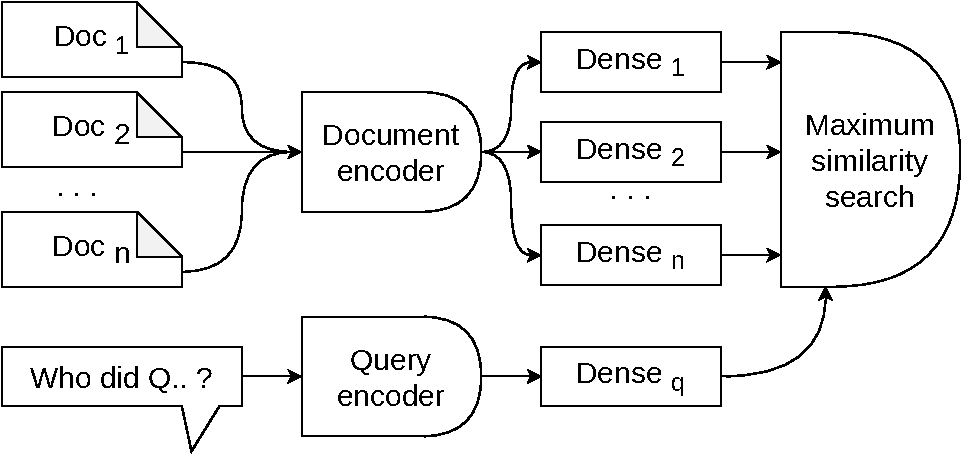
\includegraphics[width=0.7\linewidth]{img/split_concept_1.pdf}

    \caption{Conceptualized overview of retrieval on whole documents. Not actually used in practice with dense vector representations.}
    \label{fig:split_concept_1}
\end{figure}

The issue with this approach is that the pre-trained language models do not capture the meaning of the whole document in a 768-dimensional vector well \citep{reimers2019sentence,beltagy2020longformer}.
Although it is possible to extend the dimensionality to 2048-dimensional vectors to better capture the meaning \citep{beltagy2020longformer,appalaraju2021docformer}, this creates other issues, such as spurious matches.
To alleviate this, the documents are split into \emph{spans} over which the maximum similarity search is performed, as shown in \Cref{fig:split_concept_2}.
Note that large vector approaches, i.e. TF-IDF/BM25 are an exception and can operate also on long documents, usually \citep{lv2011documents}.

\begin{figure}[ht]
    \center
    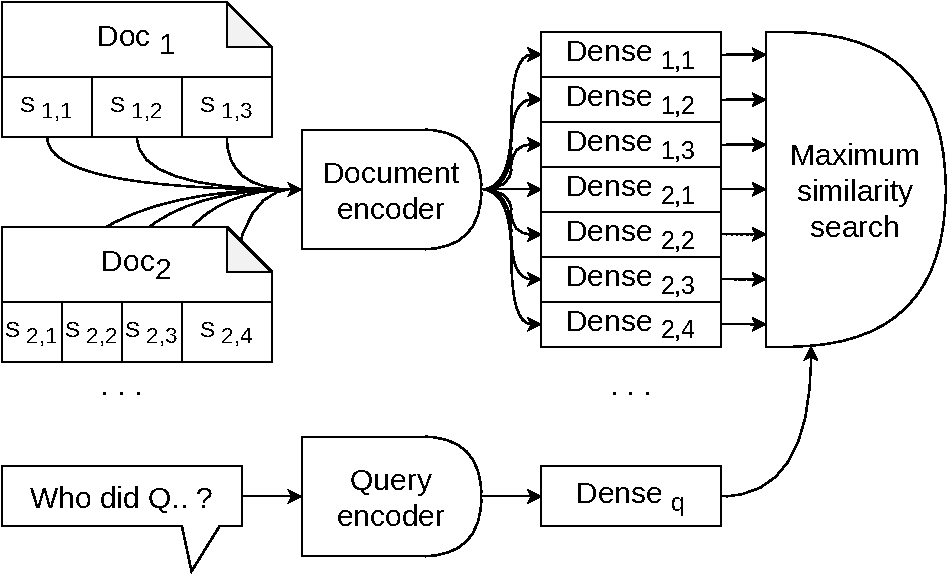
\includegraphics[width=0.7\linewidth]{img/split_concept_2.pdf}

    \caption{Conceptualized overview of retrieval on document spans.}
    \label{fig:split_concept_2}
\end{figure}

The various splitting mechanisms are described in \Cref{chapter:splitting_filtering}.
For this chapter and most of the experiments in this thesis, we use splitting by non-overlapping spans of length 100 tokens.
This is slightly suboptimal, but commonly used \citep{karpukhin2020dense}.

\subsection{Evaluation}

There are a plethora of ways of evaluating document retrieval systems, as surveyed briefly by \citet{bama2015survey}.
To evaluate retrieval performance we use two metrics.
For dimension reduction (\Cref{chapter:dim_reduction}) we compute \textit{R-Precision} averaged over queries $q_i$: (relevant documents among top $k$ passages in $Z$)$/r$, $k$ = number of passages in relevant documents, in the same way as \citet{petroni2021kilt}.
For splitting and filtering (\Cref{chapter:splitting_filtering}) we compute \textit{top-10 accuracy} averaged over queries $q_i$: $\mathbf{1}_{r\,\cap\,(arg\,top-10_{d_j}\,\text{sim}(q_i, d_j)) \neq \emptyset}$.\footnote{$\mathbf{1}$ is the indicator function. Top-k accuracy for a single query is 1 if the top k retrieved documents contain at least one relevant document, otherwise 0.}
The reason for using R-Precision is that it is commonly used \citep{sakai2007reliability,bama2015survey}.
This metric can, however, not be used for the splitting and filtering experiments because there we modify the number of relevant passages which makes the comparison even within one experiment impossible and could lead to false conclusions.
Using two metrics in one thesis is further warranted by the lack of necessity to compare results between the two chapters.

\subsection{Similarity Functions}

There is no unified mathematical definition of what a similarity function is.
A working definition for our context of dense document encoding retrieval is that it is a function which is high for similar vectors and low for dissimilar ones:
\begin{gather*}
    \text{sim}: \mathbb{R}^d \times \mathbb{R}^d \rightarrow \mathbb{R}
\end{gather*}

A common approach is to take the inverse or the negation of the $L^2$ (Euclidean) distance.
Note that in contrast to the $L^2$ distance, which is non-negative, the similarity function is unbounded.
Another mathematical function often used for similarity is the inner product (vector dot product).
\begin{align*}
    L^2(a,b)                  & = \sqrt{(a-b)^2} = \sqrt{{\mathlarger{\mathlarger\Sigma}}^d_1 (a_i-b_i)^2} \\
    \text{sim}_{L^2}(a,b)     & = -L^2(a,b) = -\sqrt{{\mathlarger{\mathlarger\Sigma}}^d_1 (a_i-b_i)^2}     \\
    \text{sim}_\text{IP}(a,b) & = \text{IP}(a,b) = {\mathlarger{\mathlarger\Sigma}}^d_1 (a_i\cdot b_i)
\end{align*}

A key property of these two functions is that they are recursively decomposable \citep{JDH17} and various improvements can be used to speed up the retrieval.
There are other metrics, such as the cosine distance (equivalent to the inner product in normalized space), $L^1$, $L^\infty$, Canberra \citep{lance1966computer}, Bray-Curtis dissimilarity \citep{thakur2019analysis}, Jensen-Shannon divergence \citep{lin1991divergence}, Mahalanobis distance \citep{mahalanobis1936generalized} and many others \citep{vijaymeena2016survey,joshi2019dissimilarity,sitikhu2019comparison}.
We focus only on the inner product (IP) and the $L^2$ distance as the similarity function because either the other metrics are not widely adopted in the community or the FAISS framework does not fully support them.\footnote{For example, the cosine similarity can be used only for normalized vectors, which would prevent us from experimenting with the unnormalized vectors.}
See \Cref{tab:dataset_example} for vector similarities between specific textual spans.

\begin{table}
    \center
    \renewcommand{\arraystretch}{1.5} % should affect only this table
    \begin{tabular}{p{7.5cm}lc}
        \toprule
        \textbf{Test}                                                                                             & \textbf{Type}               & \textbf{Query Similarity} \\
        \midrule
        % 8362
        \textbf{HotpotQA}:\newline The district that the village of Asamang is located in was split on what date? & Query                                                   \\
        \cmidrule{2-3}
        % 1186011
        Asamang is a village in the Atwima Nwabiagya district, a district in the Ashanti Region of Ghana.
                                                                                                                  & Relevant span
                                                                                                                  & \makecell[tl]{IP $= 0.476$                              \\ $L^2 = -1.023$} \\
        % 1633522
        The Atwima Nwabiagya District formerly the Atwima District is one of the twenty-seven (27) districts in the Ashanti Region of Ghana. Its capital is Nkawie. In 2003, part of the district was split off by a decree of president John Agyekum Kufuor on November 12, 2003, to form the new Atwima Kwanwoma District and Atwima Mponua District.
                                                                                                                  & Relevant span
                                                                                                                  & \makecell[tl]{IP $= 0.440$                              \\ $L^2 = -1.058$} \\
        % 194146
        Lowery married filmmaker Augustine Frizzell in 2010. As of 2013, they live in Dallas. Lowery identifies as an atheist, and has been a vegan since around 1996.
                                                                                                                  & Irrelevant span
                                                                                                                  & \makecell[tl]{IP $= -0.176$                             \\ $L^2 = -1.534$} \\
        \midrule
        % 1971
        \textbf{Natural Questions}:\newline minister of energy and power development in zimbabwe                  & Query                                                   \\
        \cmidrule{2-3}
        % 960312
        The Ministry of Energy and Power Development is a government ministry, responsible for energy and electricity in Zimbabwe. The incumbent minister is Ambassador Joram Gumbo.
                                                                                                                  & Relevant span
                                                                                                                  & \makecell[tl]{IP $= 0.758$                              \\ $L^2 = -0.696$} \\
        % 40621
        both in June 2017, in protest at Trump's decision to withdraw the United States from the Paris Agreement on climate change.
                                                                                                                  & Irrelevant span
                                                                                                                  & \makecell[tl]{IP $= -0.023$                             \\ $L^2 = -1.430$} \\
        \bottomrule
    \end{tabular}
    \caption{Example of questions from HotpotQA and Natural Questions. Similarity is measured on centered and normalized embeddings from DPR-CLS. Higher always means more similar ($L^2$ is for this reason negated).}
    \label{tab:dataset_example}
\end{table}


\subsection{Data} \label{subsec:model_and_data}

As the knowledge base we use documents from English Wikipedia dump 2019 and follow the setup described by \citet{petroni2021kilt}.
We mark spans (original articles split into 100 token pieces, 50 million in total) as relevant for a query if they come from the same Wikipedia article as one of the provenances.\footnote{Spans of the original text which help in answering the query.}
In order to make our experiments computationally feasible and easy to reproduce we experiment with a modified version of this knowledge base where we keep only spans of documents that are relevant to at least one query from the training or validation set of our downstream tasks.
As downstream tasks, we use HotpotQA \citep{yang2018hotpotqa} for all main experiments and Natural Questions \citep{kwiatkowski2019natural} to verify that the results transfer to other datasets as well.
They are both widely used by the research community \citep{chakravarti2020towards,luo2021simple,lia2021synchronous,ding2021reasoning,gontier2022does,bonifacio2022inpars} and we chose them because of their popularity and availability within the KILT framework.
HotpotQA has been sourced through careful crowdsourcing and is aimed at multi-hop reasoning.
Natural Questions were created by aggregating and anonymizing queries issued to the Google search engine.
We show examples from the two datasets in \Cref{tab:dataset_example} together with the vector similarity between the query and selected spans.
Note that the vector similarity is higher for the relevant spans than for the irrelevant ones.

This datset preprocessing to over 2 million encoded spans for HotpotQA (see \Cref{tab:dataset_size} for dataset sizes).
The 768-dimensional embeddings (32-bit floats) of this dataset (both queries and documents) add up to 7GB (146GB for the whole unpruned dataset).


\begin{table}[ht]
    \center
    \renewcommand{\arraystretch}{1.3} % vertical padding
    \begin{tabular}{lccc}
        \toprule
        \textbf{Dataset}           & \textbf{Train queries} & \textbf{Dev queries} & \textbf{Documents} \\
        \midrule
        HotpotQA                   & 69k                    & 6k                   & 49.7 Mio.*         \\
        HotpotQA (pruned)          & 69k                    & 6k                   & 2.1 Mio.           \\
        Natural Questions (pruned) & 78k                    & 2k                   & 1.6 Mio.           \\
        \bottomrule
    \end{tabular}
    \caption{Number of training and dev queries and documents for the different datasets used. *Whole Wikipedia dump.}
    \label{tab:dataset_size}
\end{table}


\subsection{Model Comparison}

To establish baselines for uncompressed performance we use models based on BERT \citep{devlin2019bert}.
We consider (1) vanilla BERT, (2) SentenceBERT \citep{reimers2019sentence} and (3) DPR \citep{karpukhin2020dense}, which was specifically trained for document retrieval.
See \Cref{subsec:embd_model_overview} for a brief overview of how these models were trained and their differences.
To obtain document embeddings, we use either the last hidden state representation at \texttt{[CLS]} or the average across tokens of the last layer (both are commonly used to get the vector representation of the input).

Our first experiment compares the retrieval performance of the different models on HotpotQA.
The result is shown in \Cref{fig:model_intro}.
In alignment with previous works \citep{reimers2019sentence} an immediately noticeable conclusion is that vanilla BERT has a poor performance,\footnote{See \Cref{subsec:embd_model_overview} for explanation.} especially when taking the hidden state representation for the \texttt{[CLS]} token.
Next, to make the computation of experiments tractable on available hardware, we repeat the experiment using FAISS \citep{JDH17},\footnote{Parameters: {IndexIVFFlat, nlist=200, nprobe=100}.} which is a framework for fast approximate similarity search.
We find that the performance loss across models is systematic, which warrants the use of this approximation for comparisons and all our following experiments will use FAISS on the DPR-CLS model.\footnote{The authors of DPR also used FAISS in their paper when presenting results.}

\begin{figure}[ht]
    \center
    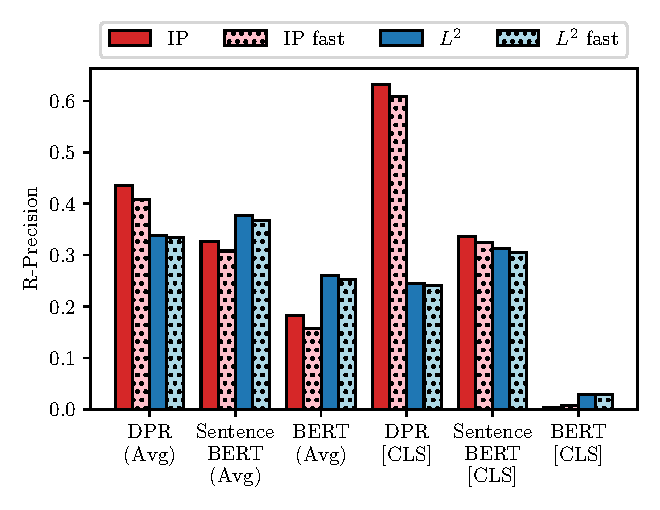
\includegraphics[width=0.7\linewidth]{img/model_intro.pdf}

    \captionsetup{type=figure}\caption{Comparison of different BERT-based embedding models and versions when using faster but slightly inaccurate nearest neighbour search. \textbf{[CLS]} is the specific token embedding from the last layer while \textbf{(Avg)} is all token average.}
    \label{fig:model_intro}
\end{figure}

\begin{figure}[ht]
    \center
    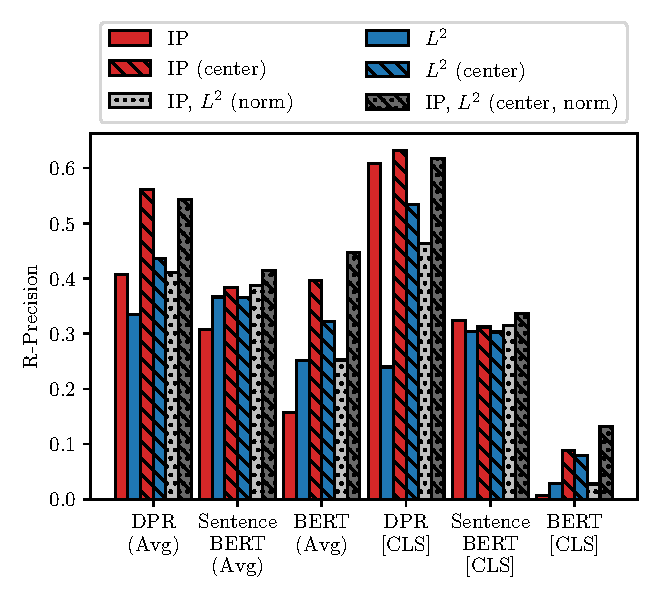
\includegraphics[width=0.7\linewidth]{img/model_normalization.pdf}

    \caption{Effect of data centering and normalization on performance  (evaluated with FAISS).}
    \label{fig:model_normalization}
\end{figure}

\begin{figure}[ht]
    \center
    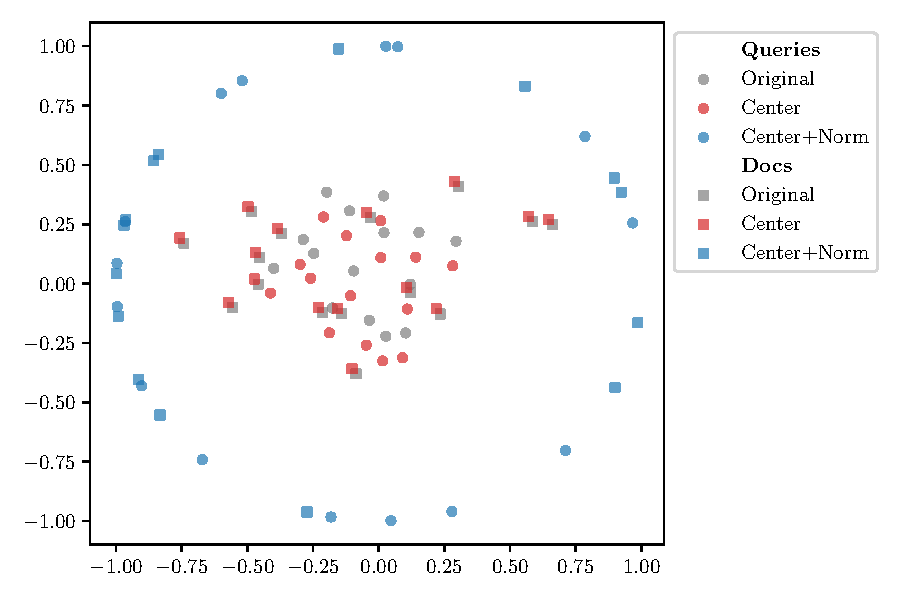
\includegraphics[width=0.9\linewidth]{img/norm_examples.pdf}

    \caption{First two dimensions of 15 random queries and 15 random documents and their positions after preprocessing.}
    \label{fig:norm_example}
\end{figure}

To provide further intuition to why normalization may help we show specific query and document vectors in \Cref{fig:norm_example}.
Note that while the centering of one dimension is independent of centering of the other dimensions, the normalization of one dimension is dependen on other dimensions.
For this reason, we consider only the first two dimensions of the 768-dimensional vectors.
Also note that the preprocessing of queries is independent on the preprocessing of documents.
For this reason we can see that while centering preserves the shape, it moves the queries down-left, while the documents are shifted up-left.
The normalization sets the vectors along a hypersphere (a circle in 2D case).
Formally, this slightly reduces the information content of one vectors by almost one dimension.\footnote{If we know 767 dimensions $d_1, \ldots d_{767}$, we can deduce that the last element is going to be $d_{768} = \pm \sqrt{1-\sum_1^{767} d_i^2}$. If we used polar coordinates, we would need exactly 767 numbers because the magnitude is always 1.}
With this, the vectors are differentiated only by the angles and not their absolute magnitude.
This further allows us to unify the ordering given by $L^2$, the inner product and the cosine similarity.

\subsection{Embedding Model Overview} \label{subsec:embd_model_overview}

In this subsection, we provide a brief background of the design and training of the pre-trained models used for embedding spans: BERT, SentenceBERT and DPR.
While many more models exist, we chose these three because they are commonly used and the later two are based on the first one and vastly improve on it.

\subsubsection{BERT}

Bidirectional Encoder Representations from Transformers (BERT \citep{bert}) is based on the encoder part of the transformers \citep{vaswani2017attention} architecture (multiple blocks of embedding, multihead self-attention, feed forward and layer normalization).
The goal is to obtain \emph{some} representation of the input such that it can be finetuned and used for various other tasks either directly or with a small degree of finetuning.\footnote{The original paper used natural language understanding but it has been applied for a plethora other NLP tasks \citep{qu2019bert,yang2020bert,kaliyar2021fakebert,liu2019fine,liu2019text,hakala2019biomedical,rongali2020don,he2020establishing,gao2019target,munikar2019fine}. Because of its popularity, it has also been adopted into other languages \citep{delobelle2020robbert,chan2020german,sido2021czert,cui2021pre,virtanen2019multilingual,wang2020extending,dumitrescu2020birth,de2019bertje} and exists in a multilingual version as mBERT.}
The way this is done is by pretraining the model on large amounts of data on two tasks: language modelling and next-sentence prediction.
Consider the following two inputs (each on separate line):

\medskip
\resizebox{\linewidth}{!}{%
    \begin{minipage}{17cm}
        \begin{center}
            \emph{[CLS] [MASK] hedgehog fell [MASK] . [SEP] Gabriel García Márquez was born in 1927 . [SEP] \hspace{0.01cm} \text{}} \\
            \emph{[CLS] He grew up with [MASK] grandparent . [SEP] His grandfather used to be a colonel . [SEP]} \\
        \end{center}
    \end{minipage}%
}
\smallskip

The goal of masked language modelling is to predict the masked tokens from context (variable number of tokens were masked, 15\%).
For the two examples the gold answers are \emph{The}, \emph{asleep} and \emph{his}, respectively.
The goal of next sentence prediction is to determine whether the second sentence follows the first.
In the first example the sentences are not probable to be consecutive while in the second example they are.
For the pretraining the last block in the model is followed up with classification layers.
Notice the special tokens \texttt{[CLS]}, \texttt{[MASK]} and \texttt{[SEP]} which provide some structure to the input.
Furthermore, BERT does not use whole tokens as the input units but subword made by WordPiece \citep{wu2016google} and therefore the vocabulary consists of parts of words (this is not depicted in the example).

\subsubsection{SentenceBERT}

While both BERT and Roberta \citep{liu2019roberta} improved the state of the art for tasks relying sentence pair similarity, the main issue is that the two sentences need to be put into the model.
To find the most semantically similar sentence (to a specific one in a dataset of 50 Mio. sentences would require 50 Mio. inferences of the large model, which is highly impractical from compute resources point of view.

The authors of SentenceBERT try to alleviate this by trying to find a function $f$ for which the following holds ($\text{sim}$ is a vector similarity function, in their case cosine similarity):
\begin{gather*}
    \argmax_i \,\text{ sim}(f(s_i), f(s_j)) \quad\Leftrightarrow\quad s_i \text{ is semantically similar for } s_j
\end{gather*}

That is, they build a model which computes the embedding of the sentence such that in the new vector space, similar sentences are close together (based on cosine similarity).
We can precompute $f(s_i)$ for every sentence and during inference, we only need to compute $f(s_j)$ and run a maximum similarit search over the precomputed dataset.
The model is based on BERT but with a modified objective function, which (among others experimented with) is the following (given random positive and negative sentences $s_p$ and $s_n$):
\begin{gather*}
    \max(||f(s_i)-f(s_p)||-||f(s_i)-f(s_n)||+\epsilon, 0)
\end{gather*}

In practice, this minimizes $||f(s_i)-f(s_p)||$ while maximizing $||f(s_i)-f(s_n)||$.
The $\epsilon$ is just a stabilization constant that ensures that the difference between the two distances is at least $\epsilon$.
The model is trained on the SNLI and Multi-Genre SNLI dataset which classifies pairs of sentences with \emph{contradiction}, \emph{entailnment} and \emph{neutral}. 

\subsubsection*{Dense Passage Retrieval}

Because the DPR model is the one used for most experiments in this thesis, it is the most important.
The goal for document retrieval is to have functions $f_d$ and $f_q$ for which the following holds:
\begin{gather*}
    \argmax_i \,\text{ sim}(f_d(d_i), f_q(q_j)) \quad\Leftrightarrow\quad d_i \text{ is relevant for } q_j
\end{gather*}

Note that for BERT and SentenceBert we use $f_d = f_q$ despite text spans $d_i \in \mathcal{D}$ and $q_j \in \mathcal{Q}$ coming from different distribution.
One of the advantages of DPR is that it distinguishes these two functions.
They start with two pretrained BERT base uncased models and optimize them in the following loss using contrastive learning (given batch $i$, query $q_i$, a relevant span $p_i$ and set of negative samples $N_i$):
\begin{gather*}
    \mathcal{L}(q_i, p_i, N_i) = -\log \frac{e^{\text{sim}(q_i,p_i)}}{e^{\text{sim}(q_i,p_i)} + \sum_j e^{\text{sim}(q_i,N_{i,j})}}
\end{gather*}
Note that $q_i$, $p_i$ and $N_i$ are all the results of computations via $f_q$ and $f_d$ to which loss can be backpropagated.
This essentially computes a softmax of the following vector at the first position:
\begin{gather*}
    [\text{sim}(q_i, p_i), \text{sim}(q_i, N_{i,1}), \text{sim}(q_i, N_{i,2}), \ldots, \text{sim}(q_i, N_{i,|N_i|})]
\end{gather*}
The whole fraction is in the interval $(0,1)$.
We want the nominator to be large (high similarity with the relevant span) while the denominator to be small (low similarity with irrelevant spans).
Minimizing the negative log of this fraction pushes the fraction to be close to 1.

The positive span is easily available from the dataset while the negative spans need to be sampled carefully.
The authors discuss multiple strategies for this selection, including (1) random sampling, (2) top false output of BM25, (3) positive spans for other questions in the batch, also called in-batch negatives, and (4) the combination of them, which results in their best model.